% @file load_data.tex
% @project IAL Náhradní projekt - 05. Rovinnost grafu
% @author Vladimir Meciar (xmecia00), Ondrej Podrouzek (xpodro03)
% @brief This file is module for documentation.tex with documantation for scanner
% @changes 7.12.2022
\section{Načítání dat}

\subsection{Vstupní data}
Struktůra kterou potřebujeme načítat (graf), je definovaná jako množina vrcholů a hran. Pro naše potřeby
jsme použili uložení v textu s formátem.

\begin{lstlisting}
Vertice_id:
  - edge_to_vertice_id
  - edge_to_vertice_id
  - edge_to_vertice_id
  - edge_to_vertice_id;
\end{lstlisting}

Scanner si nastaví buffer pro zapsání čísla a začíná na stavu 0. Přečte soubor znak po znaku funkcí a dívá se na první písmeno, které je na řádku. Scanner očekává soubor v přesném formátu viz. obrázek automatu scanneru, podle kterého bude první písmeno ‚V‘ nebo ‚ ‘ (mezera) a tyto dvě možnosti jsou vyjádřeny přes switch. Pokud řádek začíná znakem ‚V‘ předpokládá, že je ve stavu 0 a kontroluje, že Vrchol je v přesném formátu. Zapíše čísla do bufferu a po konci řádku vytvoří Vrchol z id, které má zapsané v bufferu a nastaví stav na 1. Stejně pracuje pokud řádek začíná ‚ ‘ mezerou, zde se jedná o hranu. Kde očekává stav 1 (hned po zápisu vrcholu), nebo stav 2 (po zápisu hrany). Na konci zápisu hrany se dívá, jestli tento řádek nekončí ‚/n‘ čímž nastaví stav 2 a pokračuje ve čtení hran pokud řádek končí ‚;‘, který značí konec struktury vrcholu. Nastaví stav na 0 a celý cyklus se opakuje, až do konce souboru.

\begin{figure}[h]
    \centering
    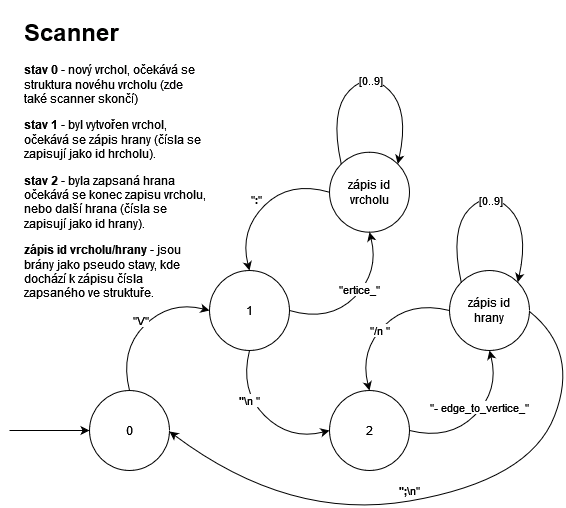
\includegraphics[width=0.9\textwidth]{doc/fig/Scanner_automat_Final.drawio.png}
    \caption{DKA}
    \label{fig:DKA}
\end{figure}


\newpage
